\documentclass[11pt,a4paper]{article}
\usepackage[margin=2.1cm]{geometry}
\usepackage{amsmath,booktabs,tabularx,xcolor,hyperref,enumitem,graphicx,float,caption}
\hypersetup{colorlinks,linkcolor=blue!50!black,urlcolor=blue!50!black}
\setlist{itemsep=1pt,topsep=2pt}
\captionsetup{font=small,labelfont=bf}
\newcommand{\code}[1]{\texttt{\small #1}}
\definecolor{bad}{HTML}{B5403A}\definecolor{good}{HTML}{2E7D4F}
% generated by scripts/backtest_peer_report.py -- do not edit
\newcommand{\PeerIcTable}{\begin{tabular}{llrrrrr}\toprule
Hedge & Signal & h & IC & $t$ & Skip a month & Beyond spread, skip \\ \midrule
carry kept & Buy the widest & 3 & +0.284 & 9.2 & +0.251 (4/4) & -- \\
carry kept & Old leverage line & 3 & +0.215 & 8.8 & +0.195 (4/4) & +0.035 ($t$ 3.0, 2/4) \\
carry kept & Peer gap + carry & 3 & +0.209 & 9.2 & +0.175 (4/4) & +0.037 ($t$ 3.7, 3/4) \\
\addlinespace
carry kept & Buy the widest & 6 & +0.338 & 7.7 & +0.313 (4/4) & -- \\
carry kept & Old leverage line & 6 & +0.258 & 7.3 & +0.242 (4/4) & +0.060 ($t$ 3.3, 2/4) \\
carry kept & Peer gap + carry & 6 & +0.243 & 7.5 & +0.217 (4/4) & +0.059 ($t$ 3.8, 3/4) \\
\addlinespace
carry kept & Buy the widest & 12 & +0.388 & 7.8 & +0.373 (4/4) & -- \\
carry kept & Peer gap + carry & 12 & +0.288 & 6.9 & +0.271 (4/4) & +0.117 ($t$ 6.6, 3/4) \\
\addlinespace
spread move & Buy the widest & 3 & +0.075 & 3.0 & +0.048 (3/4) & -- \\
spread move & Old leverage line & 3 & +0.049 & 2.5 & +0.032 (2/4) & +0.046 ($t$ 3.8, 2/4) \\
spread move & Peer gap & 3 & +0.059 & 4.0 & +0.033 (3/4) & +0.042 ($t$ 5.0, 3/4) \\
\addlinespace
spread move & Buy the widest & 6 & +0.068 & 2.0 & +0.051 (2/4) & -- \\
spread move & Old leverage line & 6 & +0.039 & 1.5 & +0.028 (1/4) & +0.073 ($t$ 3.8, 2/4) \\
spread move & Peer gap & 6 & +0.050 & 2.5 & +0.031 (3/4) & +0.063 ($t$ 4.9, 3/4) \\
\addlinespace
spread move & Buy the widest & 12 & +0.022 & 0.6 & +0.016 (2/4) & -- \\
spread move & Peer gap & 12 & +0.020 & 1.0 & +0.014 (1/4) & +0.123 ($t$ 7.4, 3/4) \\
\addlinespace
\bottomrule\end{tabular}}
\newcommand{\PeerBookTable}{\begin{tabular}{lllrrrrrrr}\toprule
Hedge & Book & Timing & Gross & Net 15 bp & Net TRACE & Sharpe & Vol & Worst DD & Cycles \\ \midrule
carry kept & Buy the widest & same & +4.7 & +4.1 & +2.5 & +0.37 & 10.9 & -24 & 3/4 \\
carry kept & Old leverage line & same & +3.2 & +2.5 & -0.3 & +0.30 & 8.6 & -21 & 3/4 \\
carry kept & Old leverage line (s-n) & same & +0.9 & +0.2 & -1.7 & +0.06 & 3.3 & -9 & 2/4 \\
carry kept & Peer gap + carry & same & +4.4 & +3.7 & +1.5 & +0.48 & 7.8 & -14 & 3/4 \\
carry kept & Peer gap + carry (s-n) & same & +1.4 & +0.7 & -1.2 & +0.33 & 2.0 & -5 & 3/4 \\
carry kept & Buy the widest & skip & +2.6 & +2.0 & +0.4 & +0.18 & 10.9 & -30 & 2/4 \\
carry kept & Old leverage line & skip & +2.0 & +1.4 & -1.0 & +0.16 & 8.8 & -26 & 3/4 \\
carry kept & Old leverage line (s-n) & skip & +0.8 & +0.1 & -1.3 & +0.02 & 3.2 & -8 & 2/4 \\
carry kept & Peer gap + carry & skip & +2.6 & +2.0 & +0.2 & +0.26 & 7.5 & -16 & 2/4 \\
carry kept & Peer gap + carry (s-n) & skip & +0.7 & -0.0 & -1.5 & -0.00 & 2.2 & -8 & 3/4 \\
\addlinespace
spread move & Buy the widest & same & +0.6 & +0.0 & -1.5 & +0.00 & 9.5 & -32 & 2/4 \\
spread move & Old leverage line & same & +0.5 & -0.2 & -2.7 & -0.02 & 9.2 & -30 & 2/4 \\
spread move & Old leverage line (s-n) & same & +0.4 & -0.3 & -2.1 & -0.07 & 3.8 & -16 & 1/4 \\
spread move & Peer gap & same & +2.1 & +1.4 & -0.8 & +0.14 & 10.2 & -17 & 2/4 \\
spread move & Peer gap (s-n) & same & +1.1 & +0.4 & -1.3 & +0.15 & 2.7 & -6 & 1/4 \\
spread move & Buy the widest & skip & -2.2 & -2.8 & -4.3 & -0.44 & 6.4 & -42 & 1/4 \\
spread move & Old leverage line & skip & -1.5 & -2.2 & -4.2 & -0.40 & 5.5 & -37 & 2/4 \\
spread move & Old leverage line (s-n) & skip & +0.2 & -0.5 & -1.8 & -0.17 & 3.0 & -16 & 1/4 \\
spread move & Peer gap & skip & -0.3 & -1.0 & -2.3 & -0.21 & 4.5 & -20 & 2/4 \\
spread move & Peer gap (s-n) & skip & +0.2 & -0.5 & -1.7 & -0.23 & 2.0 & -14 & 1/4 \\
\addlinespace
\bottomrule\end{tabular}}
\newcommand{\PeerDistressTable}{\begin{tabular}{lrrrrrr}\toprule
Book & \multicolumn{3}{c}{All bonds} & \multicolumn{3}{c}{Distressed out} \\
 & Net & Sharpe & Worst DD & Net & Sharpe & Worst DD \\ \midrule
Buy the widest & +14.3 & +0.43 & -51 & +4.1 & +0.37 & -24 \\
Old leverage line & +13.6 & +0.42 & -49 & +2.5 & +0.30 & -21 \\
Peer gap + carry & +13.0 & +0.44 & -43 & +3.7 & +0.48 & -14 \\
\bottomrule\end{tabular}}


\title{Is a bond cheap against its sector peers?\\[2pt]\large A backtest of the peer fair spread, with quarterly long-short books, 2008--2026}
\author{FundamentalQuantmental, HY Analyst}
\date{TRACE month ends January 2008 to July 2026; run 23 October 2026}

\begin{document}
\maketitle

\noindent\fcolorbox{gray}{gray!6}{\parbox{\dimexpr\linewidth-2\fboxsep-2\fboxrule}{%
\textbf{The answer}
\begin{enumerate}
\item \textbf{\color{good}The peer gap ranks bonds within a spread level.} Hold the spread level fixed and skip a month. The rank IC of the peer gap is then $+0.04$ at 3 months, $+0.06$ at 6 and $+0.12$ at 12, with $t$ above 3. It is positive in 3 of the 4 stress windows at every horizon.
\item \textbf{\color{bad}The peer gap alone forecasts little.} With the carry hedged out (DTS hedge) and a month skipped, its IC is $+0.03$ at 3 and 6 months and $+0.01$ at 12. The same-month IC is about twice as large; the bid-ask bounce makes the difference.
\item \textbf{\color{good}Carry is where the money is.} With carry kept and 15~bp of cost, the peer-gap-plus-carry book earns $+3.7\%$ a year after cost (Sharpe 0.48, worst drawdown $-14\%$). ``Buy the widest'' earns $+4.1\%$ (Sharpe 0.37, worst drawdown $-24\%$). The peer gap buys a smoother path, not more return.
\item \textbf{\color{bad}The forecast sizes are wrong.} The calibration slope of realised on predicted return is $-0.10$ to $+0.13$. A slope of 1 would mean the sizes are right. Use the forecast as a rank, never as a size.
\item \textbf{\color{bad}One quarter makes the spread-move book.} The quarter held through March 2020 earns $+37.8\%$. Without it the spread-move peer book loses $0.65\%$ a year.
\item \textbf{Distressed bonds stay out.} With bonds at 1{,}000~bp and wider, the carry books earn 13 to 14\% a year with drawdowns of $-43\%$ to $-51\%$. That is the default premium, not the signal.
\end{enumerate}
\textbf{What to do next.} Use the peer gap as a tie-breaker inside a carry book, not as a stand-alone trade. Fix the forecast size before any position is sized from it.}}

\section{The question}
The analyst calls a bond cheap when it pays more than bonds of the same sector, rating and maturity. This document tests that call on history. It asks four questions:
\begin{enumerate}
\item Does a bond that is cheap against its peers earn more afterwards?
\item Does that hold once spread level is fixed, so the test does not reward plain carry?
\item Does a book that buys the cheap bonds and sells the rich ones make money after trading cost?
\item Does the forecast size match the realised size?
\end{enumerate}
Where the work lives:
\begin{itemize}
\item \code{scripts/backtest\_peer\_line.py}: the run.
\item \code{hy/backtest.py}: the formulas, with tests.
\item \code{scripts/backtest\_peer\_report.py}: this document's figures and tables.
\item \code{docs/decisions/2026-10-23-peer-fair-spread.md}: the decision page.
\end{itemize}

\section{Data and universe}
\begin{enumerate}
\item \textbf{Bonds.} Every TRACE high yield bond each month end, January 2008 to July 2026: 223 months. The universe rules are those of the earlier alpha backtest (\code{backtest\_alpha.pdf}): grade H at that month end, fixed coupon, not convertible, priced from trades of \$100k par or more in the last 7 days.
\item \textbf{No look-ahead.} Every input carries \code{available\_at}. A guard stops the run if an input is dated after the decision time. The sector is the GICS sector on that date. The rating is the S\&P rating on that date where one is on file (to February 2017); after that, a rating class implied by leverage, with cut-offs fitted only on earlier months.
\item \textbf{Distressed bonds out.} A bond with a spread of 1{,}000~bp or more at formation is out (\code{hy.backtest.not\_distressed}). This removes 17{,}442 of 287{,}720 bond-months at 3 months (6\%). Above 1{,}000~bp a bond trades on recovery, not on spread, and the hedge ratio $s/S$ becomes too large to mean anything (Figure~\ref{fig:anatomy}, right).
\item \textbf{Sample.} 270{,}278 bond-months at 3 months, 275{,}106 at 6 months and 556{,}629 at 12 months.
\end{enumerate}

\section{The signal: the peer fair spread}
Each month, put every bond in a cell: GICS sector $\times$ rating class (IG, BB, B, CCC) $\times$ maturity bucket (under 3 years, 3 to 7, 7 and over). The fair spread is the median spread of the other issuers' bonds in the cell:
\begin{equation}
s^{fair}_i = \operatorname{median}_{j \in cell(i),\ j \ne i} s_j, \qquad ESP_i = \log s_i - \log s^{fair}_i .
\end{equation}
\textit{Intuition: a bond is fair when it pays what bonds of the same sector, rating and maturity pay.}

A cell needs 5 other issuers. A smaller cell falls back to rating $\times$ maturity, then sector $\times$ maturity, then maturity alone. The issuer's own bonds never count as its peers. $ESP > 0$ means the bond pays more than its peers: cheap.

\section{The forecast}
The gap to the peers closes at a speed $\rho$ per month. $\rho$ comes from past months only: one AR(1) slope pooled across issuers. The prior $0.85^{1/3}$ a month holds until enough pairs exist (from November 2008). Two forecasts, one per hedge:
\begin{align}
\hat\alpha^{move}_i &= D_i\,(1-\rho^{h})\,(s_i - s^{fair}_i) - c, \\
\hat\alpha^{carry}_i &= D_i\,(1-\rho^{h})\,(s_i - s^{fair}_i) + (s_i - S)\,\tfrac{h}{12} - c .
\end{align}
\textit{Intuition: the part of the gap that closes before the exit, times the price move per unit of spread; with carry kept, add the extra spread the bond pays over the index while it is held.}

\noindent $D$ is modified duration, $h$ the horizon in months, $S$ the HY benchmark spread, and $c$ the round-trip cost. The old leverage line (\code{fair\_line\_net}) uses the carry form with a different $s^{fair}$. ``Buy the widest'' ranks by $s$ alone.

\section{The realised return}
For each bond, from formation to $h$ months later (or to its last trade, if it stops trading):
\begin{equation}
r = \underbrace{\frac{P_{end} - P_0 + 100\,c_{pn}\,\tau}{P_0}}_{\text{price + coupon}} \;-\; \underbrace{\big(y_T\tau - D\,\Delta y_T\big)}_{\text{matched Treasury}} \;-\; \beta\,\underbrace{\big(S\tau - D\,\Delta S\big)}_{\text{HY index}} \;-\; c .
\end{equation}
Two hedges:
\begin{itemize}
\item \textbf{Spread move only:} $\beta = s/S$, the DTS hedge. The bond's carry $s$ and the hedge's carry $\beta S$ cancel. What is left is the bond's spread move against $\beta$ times the index move.
\item \textbf{Carry kept:} $\beta = 1$. The bond keeps its carry over the index, $s - S$.
\end{itemize}
A bond below a price of 50 trades flat: no coupon accrues.

\begin{figure}[H]\centering
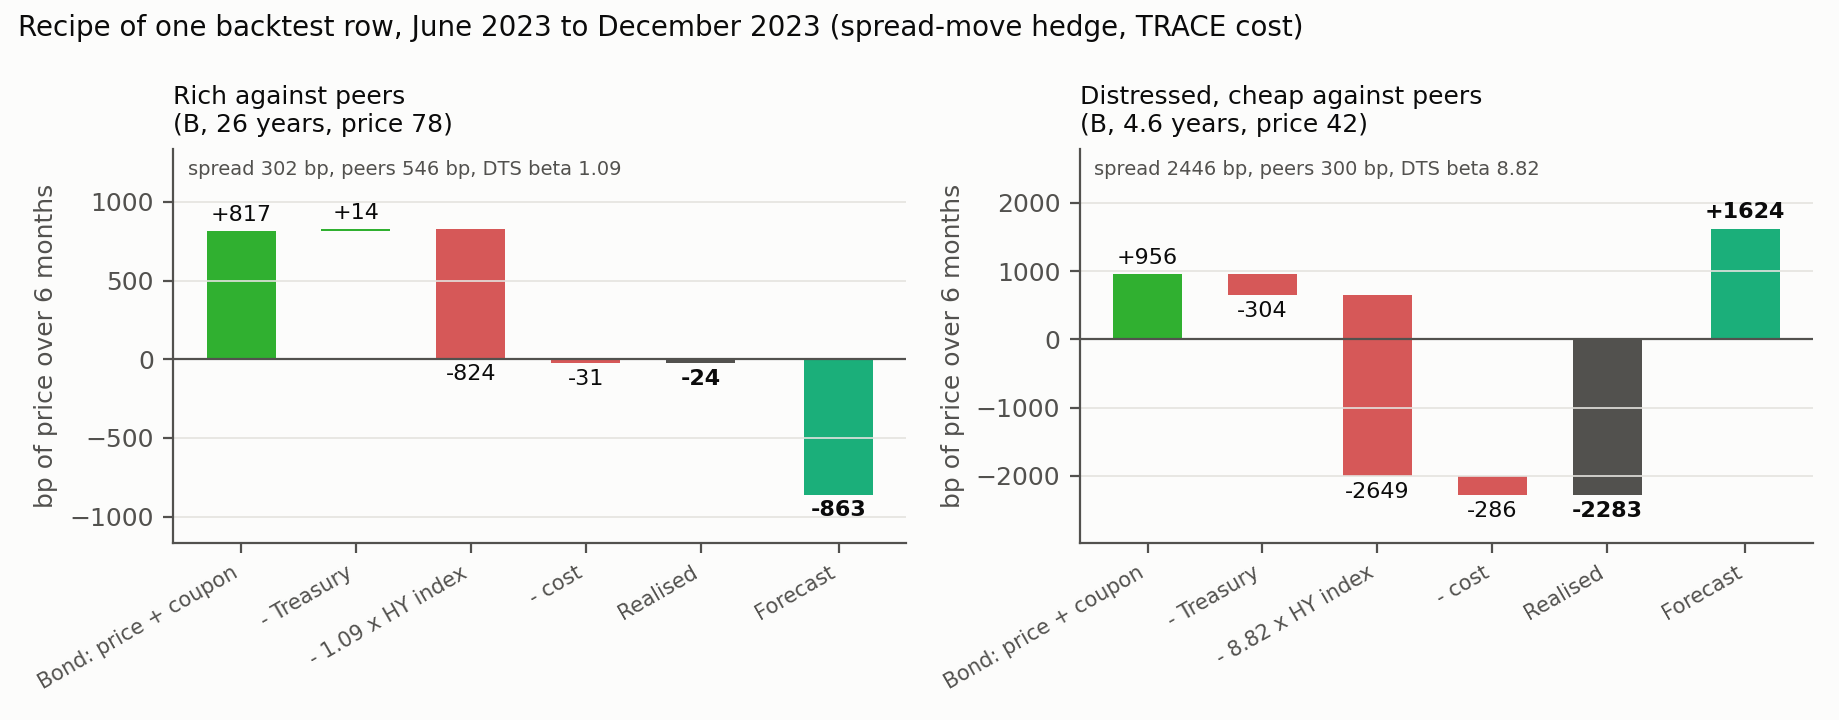
\includegraphics[width=\linewidth]{figures/peer_anatomy.png}
\caption{\label{fig:anatomy}One row of the backtest, built term by term. Left: a bond rich against its peers. The forecast ($-863$~bp) has the right sign but is 36 times too large. Right: a distressed bond at a price of 42. The bond itself rose 9.6\%, but the DTS hedge sold 8.8 times its weight in the index while the index rallied. This is why distressed bonds are out.}
\end{figure}

\section{Trading cost}
\textbf{Main case: 15~bp of price per round trip,} for every bond. This is the top of the 12 to 15~bp range that the user reports for getting in and out.

\textbf{Sensitivity: the TRACE proxy.} The proxy is each bond's bid-ask spread in TRACE that month, as a share of price. Distressed bonds out, it has a median of 24~bp and a mean of 37~bp. It rises with spread: 17~bp below 200~bp of spread, 39~bp at 700 to 1{,}000~bp. It falls over time: a median of 45~bp in 2008--2012, 19~bp in 2023--2026. The proxy uses every trade, small retail trades included, so it may overstate what an institutional desk pays.

\textbf{How the books pay it.} Each quarter, a bond that enters a leg pays one round trip, because it will leave later. A bond that stays pays nothing. About 50 to 58\% of the names change each quarter. At 15~bp this costs 0.6 to 0.7 points a year. The full-turnover rule, which charges every bond every quarter, is in the summary files as a stricter check.

\section{How the backtest scores a signal}
\begin{enumerate}
\item \textbf{Rank IC.} Each month, the Spearman correlation between the forecast and the realised return, after cost. The mean over 223 months, with a $t$-statistic corrected for the overlap of $h$-month returns (Newey--West, $h-1$ lags).
\item \textbf{Beyond spread.} Each month, take out of the realised return its linear fit on the spread rank. Score the forecast against what is left. This answers: does the signal add anything that plain spread level does not?
\item \textbf{Skip a month.} Form the forecast at $t$; earn from $t+1$. One month-end price sets both the gap and the start of the return. A noisy price makes a bond look cheap and then ``recover''. Skipping a month removes that shared noise.
\item \textbf{Stress windows.} The IC in each of four windows: 2008--09, 2015--16, 2020 and 2022. The bar of \code{CLAUDE.md}: positive in at least 3 of the 4.
\item \textbf{Size.} The Mincer--Zarnowitz slope $b$ of realised on forecast. $b = 1$ means the forecast size is right.
\end{enumerate}

\section{Results: ranking}
\begin{table}[H]\centering\small
\PeerIcTable
\caption{Rank IC after 15~bp of cost, distressed bonds out. ``Skip a month'' shows the IC and, in brackets, the stress windows with a positive IC. ``Beyond spread, skip'' shows the IC after spread level is taken out, with a month skipped. At 12 months the cache holds no old-line forecast.}
\end{table}

\begin{figure}[H]\centering
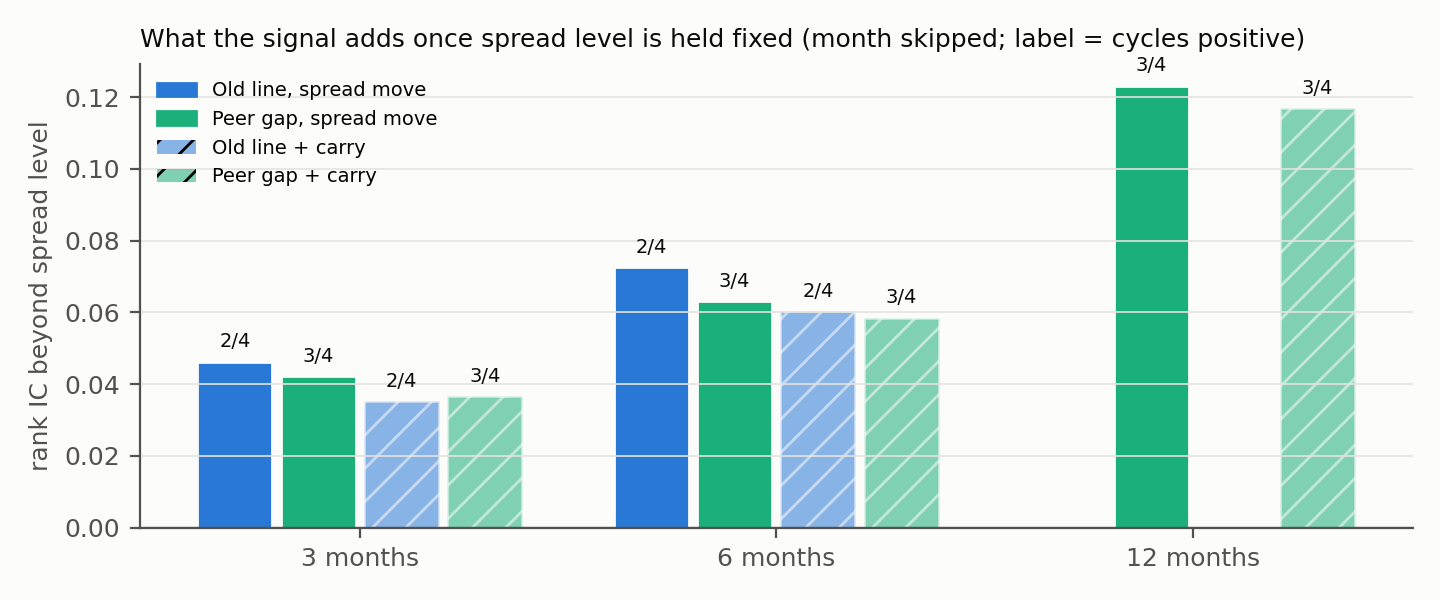
\includegraphics[width=0.85\linewidth]{figures/peer_beyond.png}
\caption{What each signal adds once spread level is held fixed, with a month skipped. The label on each bar is the number of stress windows with a positive IC. The peer gap reaches 3 of 4 at every horizon; the old leverage line reaches 2 of 4.}
\end{figure}

\noindent What the table says:
\begin{enumerate}
\item \textbf{With carry kept, every signal ranks well,} because carry ranks well: ``buy the widest'' has the highest IC (0.28 to 0.39). The carry forecasts rank slightly below it.
\item \textbf{With carry hedged out, no signal ranks well on its own.} With a month skipped the ICs are $+0.01$ to $+0.05$, and none is positive in all four stress windows.
\item \textbf{Beyond spread, the peer gap adds a little and holds across cycles.} Its edge grows with the horizon. The old line adds a similar amount but in fewer stress windows.
\item \textbf{The size is wrong everywhere.} Mincer--Zarnowitz slopes: peer gap $+0.01$ (spread move) and $+0.13$ (carry kept) at 3 months, and $-0.10$ (spread move) at 12; ``buy the widest'' $-0.10$ and $+0.08$ at 3 months.
\end{enumerate}

\section{Results: quarterly long-short books}
\textbf{Construction.} At each quarter end (March, June, September, December), rank the bonds by the forecast. Two books:
\begin{itemize}
\item \textbf{Decile:} long the top tenth, short the bottom tenth, equal weight.
\item \textbf{Spread-neutral:} split the bonds into 5 groups by spread. Inside each group, long the top fifth and short the bottom fifth of the forecast. Both legs then carry about the same spread. A pure spread signal keeps about a fifth of its premium in this book (\code{tests/test\_backtest.py}), so the neutralisation is close but not exact.
\end{itemize}
Hold 3 months, then form again: no overlap. Each leg is hedged as in Section 5.

\begin{figure}[H]\centering
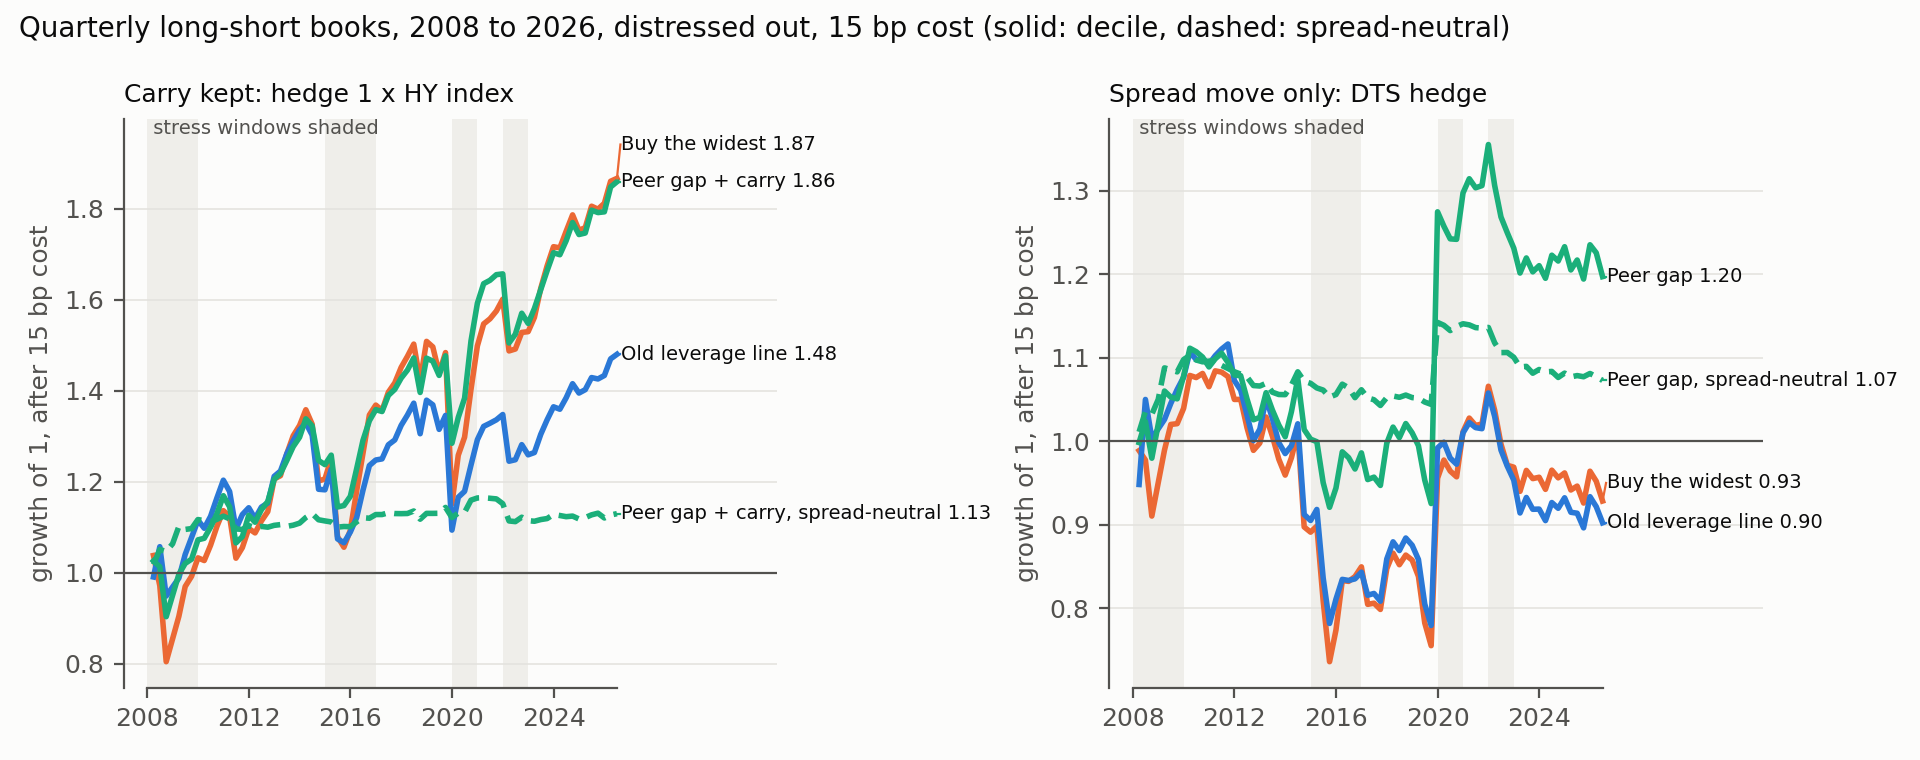
\includegraphics[width=\linewidth]{figures/peer_wealth.png}
\caption{Growth of 1 in each book, after 15~bp of cost, distressed bonds out. Left: carry kept. Right: spread move only. The jump in the right panel is the quarter formed at the end of December 2019 and held through March 2020.}
\end{figure}

\begin{table}[H]\centering\scriptsize\setlength{\tabcolsep}{4pt}
\PeerBookTable
\caption{Quarterly books, distressed bonds out. Gross: before cost. Net 15~bp: after the main cost. Net TRACE: after the TRACE proxy. Sharpe, volatility, worst drawdown and stress windows are for the 15~bp net. All returns in \% a year. (s-n): spread-neutral.}
\end{table}

\begin{figure}[H]\centering
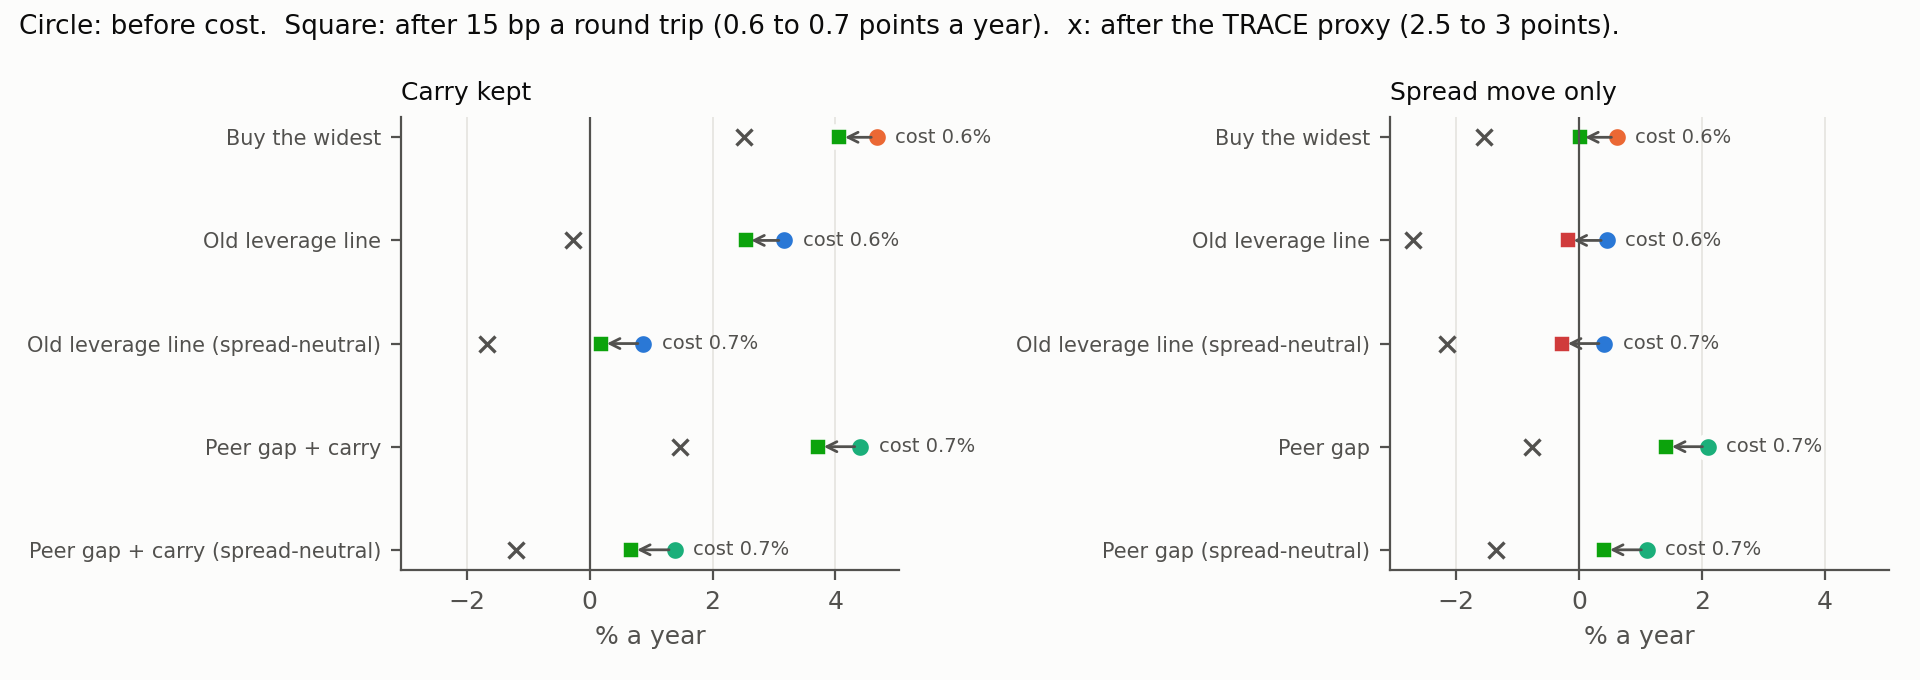
\includegraphics[width=\linewidth]{figures/peer_cost.png}
\caption{Each book's return before cost (circle), after 15~bp (square) and after the TRACE proxy (x). At 15~bp most carry books stay positive. At the TRACE proxy almost every book loses.}
\end{figure}

\noindent What the books say:
\begin{enumerate}
\item \textbf{The best book keeps carry.} Peer gap plus carry, decile: $+3.7\%$ a year after 15~bp, Sharpe 0.48, worst drawdown $-14\%$, positive in 3 of 4 stress windows. ``Buy the widest'': $+4.1\%$, Sharpe 0.37, worst drawdown $-24\%$. Both lose in the 2022 window ($-6.3\%$ and $-4.3\%$ a year).
\item \textbf{The peer gap improves the path, not the return.} It earns about 0.4 points a year less than the widest bonds. It does so with a higher Sharpe and a drawdown 10 points smaller.
\item \textbf{The spread-neutral books are nearly flat.} Peer gap plus carry, spread-neutral: $+0.7\%$ a year, volatility 2\%, worst drawdown $-5\%$. This is the pure peer-gap edge once carry is taken out. It is real, but small.
\item \textbf{The spread-move books depend on March 2020.} The peer decile book earns $+1.4\%$ a year, but one quarter earns $+37.8\%$. Its long leg made $+34\%$ while the market crashed. A likely cause: the long leg pays higher spreads, so its DTS hedge shorts more index, and the book is net short the market. This is not verified. Without that quarter the book loses $0.65\%$ a year.
\item \textbf{Skip a month and the edge halves.} Peer gap plus carry, decile, skip a month: $+2.0\%$ after 15~bp (Sharpe 0.26). ``Buy the widest'': $+2.0\%$ (Sharpe 0.18).
\end{enumerate}

\section{Distressed bonds: before and after}
\begin{figure}[H]\centering
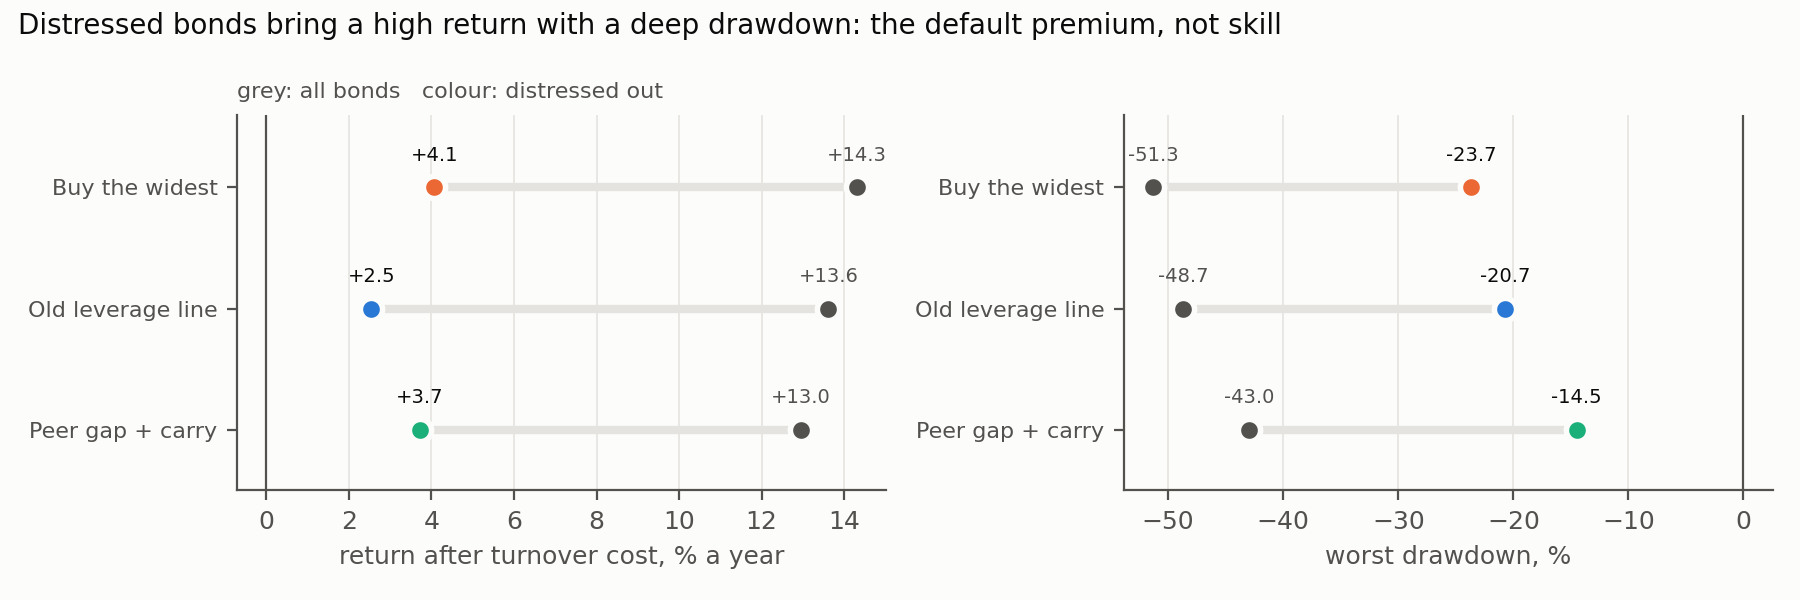
\includegraphics[width=\linewidth]{figures/peer_distressed.png}
\caption{Carry-kept decile books with all bonds (grey) and with distressed bonds out (colour). With distressed bonds in, return rises by about 10 points a year and the worst drawdown doubles.}
\end{figure}
\begin{table}[H]\centering\small
\PeerDistressTable
\caption{Carry-kept decile books, same month, after 15~bp of cost: all bonds against distressed bonds out. Net in \% a year; worst drawdown in \%.}
\end{table}
\noindent The extra return with distressed bonds in is the default premium. The long leg holds the widest bonds, and the hedge (one unit of the index) does not cover their default risk. The drawdowns of $-43\%$ to $-51\%$ show what the premium costs. No signal in this test can tell which distressed bond recovers. So the bonds stay out of the scored universe.

\section{Limits}
\begin{enumerate}
\item \textbf{Rating class after February 2017 is implied by leverage.} The S\&P rating series ends then. A wrong class puts a bond in the wrong cell.
\item \textbf{Spread is the G-spread, not the option-adjusted spread.} Most high yield bonds are callable. A bond near its call price has a G-spread that overstates its spread to worst.
\item \textbf{The cost is a flat 15~bp.} Real cost rises with spread and falls with size. The TRACE proxy shows that rise (17 to 39~bp). A flat cost flatters the wide bonds that the books buy.
\item \textbf{Equal weights and no limits.} The books have no issuer limits, no sector limits and no liquidity limits. A real book would hold fewer bonds and pay more for the small ones.
\item \textbf{The cause of the March 2020 result is not verified.} The net market exposure of each leg is not yet measured.
\item \textbf{The peer leverage for live issuers can differ from step 5.} For MGM the panel records \$31.7bn of debt against \$6.1bn in step 5. This does not touch the backtest, which uses the panel for every bond, but it touches the live memos.
\end{enumerate}

\section{How to reproduce}
\begin{enumerate}
\item \code{PYTHONPATH=. python3 scripts/backtest\_peer\_line.py --cost-bp 15} (main case).
\item \code{PYTHONPATH=. python3 scripts/backtest\_peer\_line.py --cost-bp 15} \code{--keep-distressed} (distressed comparison).
\item \code{PYTHONPATH=. python3 scripts/backtest\_peer\_line.py} (TRACE-proxy cost, distressed out).
\item \code{PYTHONPATH=. python3 scripts/backtest\_peer\_report.py} (figures and tables).
\item \code{latexmk -pdf backtest\_peer\_line.tex} in \code{docs/writeup}.
\end{enumerate}
Each run reads only cached files, so no WRDS access is needed, and finishes in under a minute. Tests: \code{tests/test\_backtest.py} covers the DTS realised return, the peer forecast, past-only $\rho$, the distressed filter, the quarter dates, the spread-neutral sort, the leg members, the turnover cost and the portfolio statistics.

\end{document}
